\begin{figure}[h!]
	\centering{
		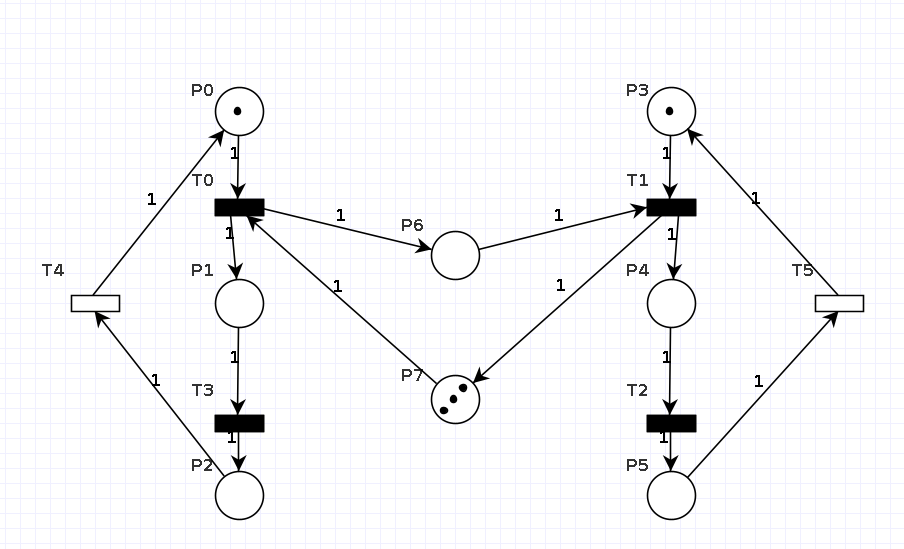
\includegraphics[width=0.67\textwidth]{img/buf.png}
	}
	\caption{Sieć reprezentująca bufor ograniczony}
	\label{zad2:graph1}
\end{figure}

\begin{figure}[h!]
	\centering{
		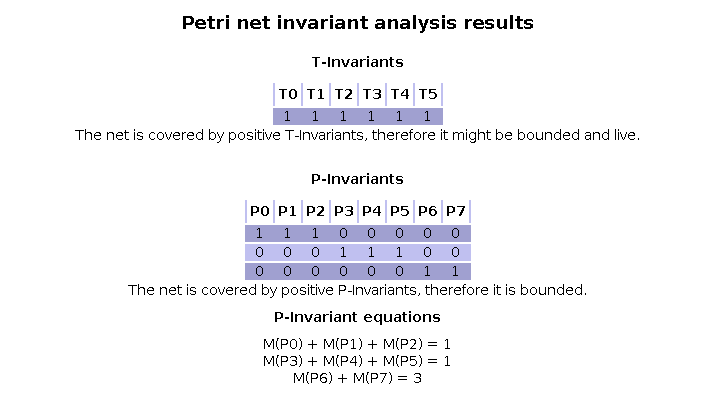
\includegraphics[width=0.67\textwidth]{img/2_1.png}
	}
	\caption{Niezminniki sieci}
	\label{zad2:graph1}
\end{figure}


\subsection{Analiza niezmienników}
Tak, sieć jest zachowawcza. 
Za pojemność bufora odpowiada ostatnie równanie.